\documentclass[conference]{IEEEtran}
\IEEEoverridecommandlockouts
% The preceding line is only needed to identify funding in the first footnote. If that is unneeded, please comment it out.
\usepackage{cite}
\usepackage{amsmath,amssymb,amsfonts}
\usepackage{algorithmic}
\usepackage{graphicx}
\usepackage{textcomp}
\usepackage{comment}
\usepackage{xcolor}
\usepackage{multirow}
\usepackage{float}
\usepackage{url}
\usepackage{graphicx}
\usepackage{caption}
\usepackage{subcaption, multicol}
\usepackage{algorithm}
\usepackage{algorithmic}
\usepackage{tikz}
\usetikzlibrary{shapes.geometric, arrows}
\def\doubleunderline#1{\underline{\underline{#1}}}

\tikzstyle{process} = [rectangle, minimum width=3cm, minimum height=1cm, text centered, draw=black, fill=orange!30]
\tikzstyle{decision} = [diamond, minimum width=3cm, minimum height=1cm, text centered, draw=black, fill=green!30]
\tikzstyle{arrow} = [thick,->,>=stealth]

\usepackage[hidelinks]{hyperref}
\def\BibTeX{{\rm B\kern-.05em{\sc i\kern-.025em b}\kern-.08em
		T\kern-.1667em\lower.7ex\hbox{E}\kern-.125emX}}
\makeatletter
\newcommand{\manuallabel}[2]{\def\@currentlabel{#2}\label{#1}}
\makeatother

\begin{document}
	\title{Passion in Action: Parallelized Smith-Waterman Implementation for GPU101 Course\\
		%A-MYCO: Prototyping the Brain of a Myco-Robot
		\thanks{Politecnico di Milano}
	}
	
	\author{\IEEEauthorblockN{Lorenzo Vergata}
		\IEEEauthorblockA{\textit{MSc in Engineering Physics} \\
			\textit{Politecnico di Milano}\\
			Milan, Italy\\
			lorenzo.vergata@mail.polimi.it}
		
	}
	
	\maketitle
	
	\begin{abstract}
		Being in the \textbf{big data} era, parallel programming is needed. This work aims to be my first step in the world of CUDA programming, trying to see if the parallel alignment of sequence of characters exceeds the serial counterpart, calculating the most similar sequence. This is done through the Smith-Waterman (SW) algorithm, by calcolating the scoring and direction matrices, then by finding the maximum score, followed by a traceback of the (most similar) sequence.\\
		After an introduction of the SW algorithm, it is described in an informal way the reason why this work exist. The challenge remains the same, but the starting code was modified a little: it is dedicated a short section on these changes. Then, after some words about GPUs architecture, the way of proceeding is provided.
	\end{abstract}
	
	\begin{IEEEkeywords}
		gpu, pia, smith-waterman, cuda, parallel programming
	\end{IEEEkeywords}
	
	\section{Introduction}
	This work is a fruit of the Passion in Action (PiA) GPU101 course at Politecnico di Milano. The students needed to implement the parallelized version of some well-known algorithm through GPU. More specifically, this code is dedicated to the Smith-Waterman (SW) algorithm, used, e.g., in bioinformatics to identify regions of similarity between two sequences. According to \cite{smith_waterman_algorithm}, the algorithm is as the following:
	\begin{algorithm}[H]
		\caption{Smith-Waterman Algorithm for Local Sequence Alignment}
		\begin{algorithmic}[1]
			\STATE \textbf{Input:} Sequences $A = a_1 a_2 \dots a_n$ and $B = b_1 b_2 \dots b_m$, similarity score function $s(a, b)$, and gap penalty $W_k$ for gap length $k$.
			\STATE \textbf{Output:} Optimal local alignment of $A$ and $B$.
			
			\STATE \textbf{Step 1: Initialization}
			\STATE Construct a scoring matrix $H$ of size $(n+1) \times (m+1)$.
			\STATE Set $H_{k0} = 0$ for $0 \leq k \leq n$ and $H_{0l} = 0$ for $0 \leq l \leq m$.
			
			\STATE \textbf{Step 2: Fill the scoring matrix}
			\FOR{$i = 1$ to $n$}
			\FOR{$j = 1$ to $m$}
			\STATE Calculate $H_{ij}$ using:\label{al}
			\[
			H_{ij} = \max\begin{cases} 
				H_{i-1, j-1} + s(a_i, b_j), \\
				\max_{k \geq 1} \{ H_{i-k, j} - W_k \}, \\
				\max_{l \geq 1} \{ H_{i, j-l} - W_l \}, \\
				0
			\end{cases}
			\]
			\ENDFOR
			\ENDFOR
			
			\STATE \textbf{Step 3: Traceback}
			\STATE Find the highest score in $H$.
			\STATE Start traceback from the cell with the highest score and continue until a cell with a score of $0$ is reached.
			\STATE Generate the local alignment based on the traceback path.
		\end{algorithmic}
	\end{algorithm}
	The extra first row and first column make it possible to align one sequence to another at any position, and setting them to 0 makes the terminal gap free from penalty.
	\begin{figure}[htbp]
		\centering
		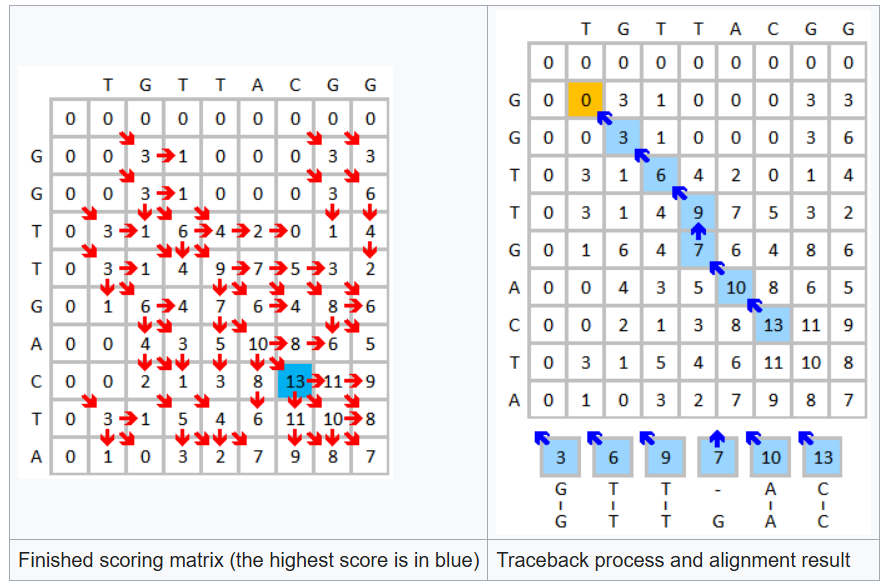
\includegraphics[width=\linewidth]{Immagine 2025-01-27 203520.png}
		\caption{The resulting alignment is \textit{GTT-AC}}
		\label{fig:boh}
	\end{figure}
	The traceback is given by the direction matrix, that has in the position \textit{i,j} a value that represent the direction pointing to the right value to reconstruct the most similar sequence. In our case we used numerical values in this matrix, as:
	\begin{itemize}
		\item 1 or 2: for pointing to left-up;
		
		\item 3: for the left;
		
		\item 4: for up direction;
		
		\item 0: no direction.
	\end{itemize}
	In our case, we had $N=1000$ sequences of length $S\_LEN=512$ consisting in $5$ nucleotides randomly chosen. At the end we have then two matrices of dimension $S\_LEN+1\times S\_LEN+1$.\\
	Of course, each step can be parallelized in harder or easier manners. Due to difficulties found in the parallelized search of the maximum, because we stored solely the maximum value per each block, only the traceback and the construction of score and direction matrices were done.

    \section{The Reason Why of This Work}
    Of course, the time dedicate in this PiA was to try to achieve the following:
    \begin{itemize}
    	\item Start to see and use some C/C++ code in order not to be scared of the course \cite{polimi_data_mining}, because due to bachelor in material science and nanotechnology, I had to start programming first by myself and then thanks to the course \cite{polimi_machine_learning};
    	
    	\item See how parallelization is done, exploiting the ways to (re-)model an algorithm;
    	
    	\item Due to syntax programming difficulties, use AI as ChatGPT, Gemini and Copilot to be able to write something working;
    	
    	\item Understand more if I like programming or not;
    	
    	\item Use the \textbf{Collatz-Weyl Generators}\cite{działa2024collatzweylgeneratorshighquality} to create the random sequences.
    \end{itemize}
    
    \section{Little Changes of the Original Code}
    The given C/C++ code was modified in order to generate the sequences through Collatz-Weyl Generators. Moreover, using as IDE CLion, the suggestions were taken into account. Nevertheless, because of the O3 optimization level, at the level of the machine almost nothing changes. Moreover, the function used to get time was reformulated in order to use a high resolution clock. Obviously, this does not affect the performance nor the effective precision due to the fact that \textit{cout} stops at the sixth significant digit by default.\\
    The seed was fixed in order to make the result be reproducible, in terms of created sequences.
    
    \section{Some Words about GPUs and CUDA}
    Thanks to their architecture, GPUs can offer w.r.t. CPUs\cite{gpu101_lecture1}:
    \begin{itemize}
    	\item Massive parallelism;
    	\item Higher throughput;
    	\item Reduced computation time;
    	\item Scalability and flexibility;
    	\item CUDA and ecosystem support.
    \end{itemize}
    CUDA organizes parallel computations in a hierarchical structure to manage and scale parallelism efficiently. The smallest unit of parallel execution in CUDA is a \textbf{thread}. Threads are grouped into \textbf{thread blocks}. All threads in a block can communicate and synchronize on tasks. Threads in a block execute 
    concurrently on a SM. When a CUDA kernel is launched, threads within each thread block are organized into groups of 32 threads called \textbf{warps}. A warp always contains 32 threads, regardless of the GPU architecture. All threads in a warp execute the same instruction at the same time (SIMT paradigm), but each thread operates on its own data 
    element. A collection of blocks forms a \textbf{grid}. Blocks in the grid are independent of each other\cite{gpu101_lecture1}.
    \begin{figure}[htbp]
    	\centering
    	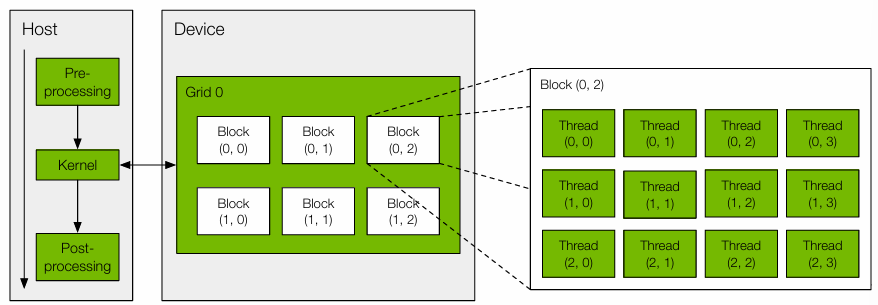
\includegraphics[width=\linewidth]{Immagine 2025-01-27 220907.png}
    	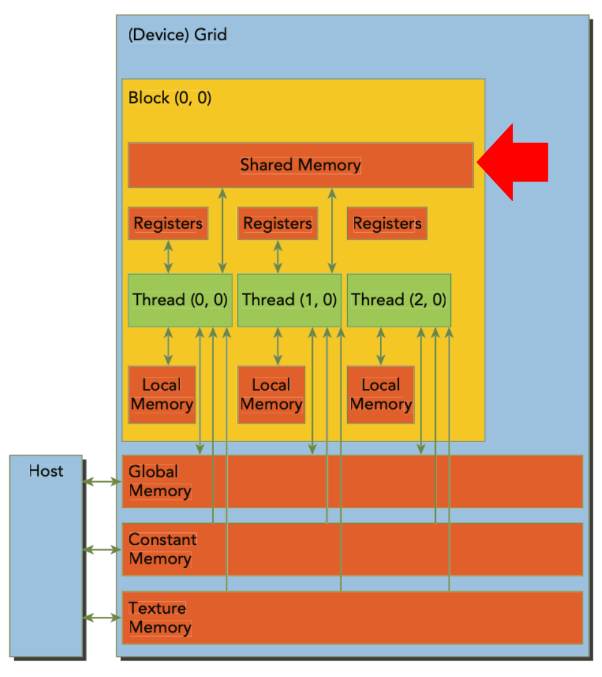
\includegraphics[width=0.7\linewidth]{Immagine 2025-01-28 093207.png}
    	\caption{Overview of the architectures we have. \textit{Host} is CPU-side, while \textit{device} is GPU-side. The accesses in the different memories play a key role to reach high performances, e.g., exploiting \textbf{coalesced access}. \cite{gpu101_lecture1}.}
    \end{figure}
    Each block is assigned to a single streaming multiprocessor (SM), i.e., computational units. SMs have CUDA cores, tensor cores, L1 cache, and registers. The latters are the fastest form of memory available to each SM. L2 cache is used as an intermediate storage layer between device memory and the SMs\cite{gpu101_lecture1}.\\
    The nearer the memory, the faster the process, and the same is with a better exploitation of the multiple of 2 (or 32) in the utilization of the resources.
    
    \section{Modus Operandi}
    We can see in the algorithm in \ref{al} that an element in position \textit{i,j} in the scoring matrix does not depend on the element in \textit{i-1,j+1}, i.e., the right-up score, so that we can make full use of the fact that if the right-up element of the score matrix exists, then we have all the elements to compute the final result in the cell \textit{i,j}. This method is a sort of parabola in terms of number of not idle threads, with only a single operative thread in the first and last computation of the score matrix, while a maximum of $S_LEN$ when computing the last element of the first row.\\
    Because of certain idle threads, the block size is of course $N$, i.e., the total number of strings, having $S_LEN$ threads for each block.\\
    Before starting the computation, the kernel uses shared memory to store the block-level maximum score and its corresponding indices. The first row and column of the score and direction matrices are initialized to zero using coalesced memory access, i.e., each thread initializes multiple matrix elements in the same row or column by incrementing by the dimension of the block (along \textit{x}).\\
    The main computation follows a diagonal traversal of the scoring matrix, and after the function \textit{dir\_score}, the maximum score and its indices are updated atomically by threads. Finally, the block-level maximum score and indices are written to global memory.\\
    After this, backtracking is performed to reconstruct the alignment path in such a way that starting from the maximum score position \((i, j)\), threads independently traverse the direction matrix.\\
    The output of the kernel provides the highest alignment score for each pair and the position where the alignment ends. For the global maximum, it was relied on a for cycle on the host, having an array of only $N$ element, saving then the index of the string that has at the end the most similar sequence.\\
    For a fair comparison, the time on the GPU version is not entirely on the GPU, but it takes account also on the memory transfers and on this final iteration for the global maximum across all the highest value in each block.
    
	\section{Experimental Results and Discussion}
	The code was executed on a NVIDIA GeForce RTX 3050 Laptop, paired with an AMD Ryzen 5600H processor, with the plug for power inserted. The maximum number of threads per block is 1024, enough for our task.\\
	The following steps were parallelized:
	\begin{itemize}
		\item Score and direction matrices: each block of threads is responsible for computing the score matrix (\(sc\_mat\)) and direction matrix (\(dir\_mat\)) for a specific sequence pair. Inside a block, threads work to compute the scores for the matrix cells using the diagonal, and the computations for the next diagonal wait until the previous one is complete;
		
		\item Traceback: After the highest score (\(max\_score\_shared\)) and its corresponding indices (\(max\_i\_shared\), \(max\_j\_shared\)) are found for a block, each thread contributes to the traceback process, building a reversed string (\(simple\_rev\_cigar\)), which records the sequence of operations required to align the query and reference sequences.
	\end{itemize}
	Unfortunately, the for cycle in the host and the copy processes from device to host and vice versa slowed the entire run, ending up in a speed up of $\approx2.5$. Nevertheless, the kernel itself compared to the serial process, sees a speed up of $\approx1000$ starting from the second run of the code.
	
	\section{Conclusion}
	For sure, the parallel programming is harder than the serialized one, and it must when high performances are needed. Also, the parallelization itself is not enough: a wise utilization of the resources must be present, because one can end up in a simple speed up that is not worth for the time invested. It is a "hardcore" programming, that even 3 AI (ChatGPT, Copilot, Gemini) cannot handle well if one has no idea of what strategy is to be implemented. In fact, they suggested a \textit{wave-fronts parallelization} where it was not possible to see any result because the shared memory capacity of 96 kB was surpassed.\\
	To make the code run faster it is needed a parallel search for the maximum, because using AI it was not possible for me to find out a true solution, as the result does not change in terms of time.
	
	\begin{comment}
		\section{Ease of Use}
		
		\subsection{Maintaining the Integrity of the Specifications}
		
		The IEEEtran class file is used to format your paper and style the text. All margins, 
		column widths, line spaces, and text fonts are prescribed; please do not 
		alter them. You may note peculiarities. For example, the head margin
		measures proportionately more than is customary. This measurement 
		and others are deliberate, using specifications that anticipate your paper 
		as one part of the entire proceedings, and not as an independent document. 
		Please do not revise any of the current designations.
		
		\section{Prepare Your Paper Before Styling}
		Before you begin to format your paper, first write and save the content as a 
		separate text file. Complete all content and organizational editing before 
		formatting. Please note sections \ref{AA}--\ref{SCM} below for more information on 
		proofreading, spelling and grammar.
		
		Keep your text and graphic files separate until after the text has been 
		formatted and styled. Do not number text heads---{\LaTeX} will do that 
		for you.
		
		\subsection{Abbreviations and Acronyms}\label{AA}
		Define abbreviations and acronyms the first time they are used in the text, 
		even after they have been defined in the abstract. Abbreviations such as 
		IEEE, SI, MKS, CGS, ac, dc, and rms do not have to be defined. Do not use 
		abbreviations in the title or heads unless they are unavoidable.
		
		\subsection{Units}
		\begin{itemize}
			\item Use either SI (MKS) or CGS as primary units. (SI units are encouraged.) English units may be used as secondary units (in parentheses). An exception would be the use of English units as identifiers in trade, such as ``3.5-inch disk drive''.
			\item Avoid combining SI and CGS units, such as current in amperes and magnetic field in oersteds. This often leads to confusion because equations do not balance dimensionally. If you must use mixed units, clearly state the units for each quantity that you use in an equation.
			\item Do not mix complete spellings and abbreviations of units: ``Wb/m\textsuperscript{2}'' or ``webers per square meter'', not ``webers/m\textsuperscript{2}''. Spell out units when they appear in text: ``. . . a few henries'', not ``. . . a few H''.
			\item Use a zero before decimal points: ``0.25'', not ``.25''. Use ``cm\textsuperscript{3}'', not ``cc''.)
		\end{itemize}
		
		\subsection{Equations}
		Number equations consecutively. To make your 
		equations more compact, you may use the solidus (~/~), the exp function, or 
		appropriate exponents. Italicize Roman symbols for quantities and variables, 
		but not Greek symbols. Use a long dash rather than a hyphen for a minus 
		sign. Punctuate equations with commas or periods when they are part of a 
		sentence, as in:
		\begin{equation}
			a+b=\gamma\label{eq}
		\end{equation}
		
		Be sure that the 
		symbols in your equation have been defined before or immediately following 
		the equation. Use ``\eqref{eq}'', not ``Eq.~\eqref{eq}'' or ``equation \eqref{eq}'', except at 
		the beginning of a sentence: ``Equation \eqref{eq} is . . .''
	\end{comment}
	\begin{comment}
		\subsection{\LaTeX-Specific Advice}
		
		Please use ``soft'' (e.g., \verb|\eqref{Eq}|) cross references instead
		of ``hard'' references (e.g., \verb|(1)|). That will make it possible
		to combine sections, add equations, or change the order of figures or
		citations without having to go through the file line by line.
		
		Please don't use the \verb|{eqnarray}| equation environment. Use
		\verb|{align}| or \verb|{IEEEeqnarray}| instead. The \verb|{eqnarray}|
		environment leaves unsightly spaces around relation symbols.
		
		Please note that the \verb|{subequations}| environment in {\LaTeX}
		will increment the main equation counter even when there are no
		equation numbers displayed. If you forget that, you might write an
		article in which the equation numbers skip from (17) to (20), causing
		the copy editors to wonder if you've discovered a new method of
		counting.
		
		{\BibTeX} does not work by magic. It doesn't get the bibliographic
		data from thin air but from .bib files. If you use {\BibTeX} to produce a
		bibliography you must send the .bib files. 
		
		{\LaTeX} can't read your mind. If you assign the same label to a
		subsubsection and a table, you might find that Table I has been cross
		referenced as Table IV-B3. 
		
		{\LaTeX} does not have precognitive abilities. If you put a
		\verb|\label| command before the command that updates the counter it's
		supposed to be using, the label will pick up the last counter to be
		cross referenced instead. In particular, a \verb|\label| command
		should not go before the caption of a figure or a table.
		
		Do not use \verb|\nonumber| inside the \verb|{array}| environment. It
		will not stop equation numbers inside \verb|{array}| (there won't be
		any anyway) and it might stop a wanted equation number in the
		surrounding equation.
		
		
		\subsection{Some Common Mistakes}\label{SCM}
		\begin{itemize}
			\item The word ``data'' is plural, not singular.
			\item The subscript for the permeability of vacuum $\mu_{0}$, and other common scientific constants, is zero with subscript formatting, not a lowercase letter ``o''.
			\item In American English, commas, semicolons, periods, question and exclamation marks are located within quotation marks only when a complete thought or name is cited, such as a title or full quotation. When quotation marks are used, instead of a bold or italic typeface, to highlight a word or phrase, punctuation should appear outside of the quotation marks. A parenthetical phrase or statement at the end of a sentence is punctuated outside of the closing parenthesis (like this). (A parenthetical sentence is punctuated within the parentheses.)
			\item A graph within a graph is an ``inset'', not an ``insert''. The word alternatively is preferred to the word ``alternately'' (unless you really mean something that alternates).
			\item Do not use the word ``essentially'' to mean ``approximately'' or ``effectively''.
			\item In your paper title, if the words ``that uses'' can accurately replace the word ``using'', capitalize the ``u''; if not, keep using lower-cased.
			\item Be aware of the different meanings of the homophones ``affect'' and ``effect'', ``complement'' and ``compliment'', ``discreet'' and ``discrete'', ``principal'' and ``principle''.
			\item Do not confuse ``imply'' and ``infer''.
			\item The prefix ``non'' is not a word; it should be joined to the word it modifies, usually without a hyphen.
			\item There is no period after the ``et'' in the Latin abbreviation ``et al.''.
			\item The abbreviation ``i.e.'' means ``that is'', and the abbreviation ``e.g.'' means ``for example''.
		\end{itemize}
		An excellent style manual for science writers is \cite{b7}.
		
		\subsection{Authors and Affiliations}
		\textbf{The class file is designed for, but not limited to, six authors.} A 
		minimum of one author is required for all conference articles. Author names 
		should be listed starting from left to right and then moving down to the 
		next line. This is the author sequence that will be used in future citations 
		and by indexing services. Names should not be listed in columns nor group by 
		affiliation. Please keep your affiliations as succinct as possible (for 
		example, do not differentiate among departments of the same organization).
		
		\subsection{Identify the Headings}
		Headings, or heads, are organizational devices that guide the reader through 
		your paper. There are two types: component heads and text heads.
		
		Component heads identify the different components of your paper and are not 
		topically subordinate to each other. Examples include Acknowledgments and 
		References and, for these, the correct style to use is ``Heading 5''. Use 
		``figure caption'' for your Figure captions, and ``table head'' for your 
		table title. Run-in heads, such as ``Abstract'', will require you to apply a 
		style (in this case, italic) in addition to the style provided by the drop 
		down menu to differentiate the head from the text.
		
		Text heads organize the topics on a relational, hierarchical basis. For 
		example, the paper title is the primary text head because all subsequent 
		material relates and elaborates on this one topic. If there are two or more 
		sub-topics, the next level head (uppercase Roman numerals) should be used 
		and, conversely, if there are not at least two sub-topics, then no subheads 
		should be introduced.
		
		\subsection{Figures and Tables}
		\paragraph{Positioning Figures and Tables} Place figures and tables at the top and 
		bottom of columns. Avoid placing them in the middle of columns. Large 
		figures and tables may span across both columns. Figure captions should be 
		below the figures; table heads should appear above the tables. Insert 
		figures and tables after they are cited in the text. Use the abbreviation 
		``Fig.~\ref{fig}'', even at the beginning of a sentence.
		
		\begin{table}[htbp]
			\caption{Table Type Styles}
			\begin{center}
				\begin{tabular}{|c|c|c|c|}
					\hline
					\textbf{Table}&\multicolumn{3}{|c|}{\textbf{Table Column Head}} \\
					\cline{2-4} 
					\textbf{Head} & \textbf{\textit{Table column subhead}}& \textbf{\textit{Subhead}}& \textbf{\textit{Subhead}} \\
					\hline
					copy& More table copy$^{\mathrm{a}}$& &  \\
					\hline
					\multicolumn{4}{l}{$^{\mathrm{a}}$Sample of a Table footnote.}
				\end{tabular}
				\label{tab1}
			\end{center}
		\end{table}
		
		\begin{figure}[htbp]
			\centerline{\includegraphics{fig1.png}}
			\caption{Example of a figure caption.}
			\label{fig}
		\end{figure}
		
		Figure Labels: Use 8 point Times New Roman for Figure labels. Use words 
		rather than symbols or abbreviations when writing Figure axis labels to 
		avoid confusing the reader. As an example, write the quantity 
		``Magnetization'', or ``Magnetization, M'', not just ``M''. If including 
		units in the label, present them within parentheses. Do not label axes only 
		with units. In the example, write ``Magnetization (A/m)'' or ``Magnetization 
		\{A[m(1)]\}'', not just ``A/m''. Do not label axes with a ratio of 
		quantities and units. For example, write ``Temperature (K)'', not 
		``Temperature/K''.
		
		\section*{Acknowledgment}
		
		The preferred spelling of the word ``acknowledgment'' in America is without 
		an ``e'' after the ``g''. Avoid the stilted expression ``one of us (R. B. 
		G.) thanks $\ldots$''. Instead, try ``R. B. G. thanks$\ldots$''. Put sponsor 
		acknowledgments in the unnumbered footnote on the first page.
	\end{comment}
	\begin{comment}
		\section*{References}
		
		Please number citations consecutively within brackets \cite{1-1955RSPTA}. The 
		sentence punctuation follows the bracket \cite{10-Hawranik1991-bc}. Refer simply to the reference 
		number, as in \cite{10-Hawranik1991-bc}---do not use ``Ref. \cite{10-Hawranik1991-bc}'' or ``reference \cite{10-Hawranik1991-bc}'' except at 
		the beginning of a sentence: ``Reference \cite{10-Hawranik1991-bc} was the first $\ldots$''
		
		Number footnotes separately in superscripts. Place the actual footnote at 
		the bottom of the column in which it was cited. Do not put footnotes in the 
		abstract or reference list. Use letters for table footnotes.
		
		Unless there are six authors or more give all authors' names; do not use 
		``et al.''. Papers that have not been published, even if they have been 
		submitted for publication, should be cited as ``unpublished'' \cite{14-7156010}. Papers 
		that have been accepted for publication should be cited as ``in press'' \cite{17-Wild266}. 
		Capitalize only the first word in a paper title, except for proper nouns and 
		element symbols.
		
		For papers published in translation journals, please give the English 
		citation first, followed by the original foreign-language citation \cite{19-PMID:18002293}.
	\end{comment}
	%\newpage
	\bibliographystyle{IEEEtran}
	% argument is your BibTeX string definitions and bibliography database(s)
	\bibliography{References}
	\vspace{12pt}
	\color{red}
	
	
\end{document}